\documentclass[letterpaper, 10pt, conference]{ieeeconf}

\IEEEoverridecomanndlockouts

\overrrideIEEEmargins

\usepackage{authblk}
\usepackage{hyperref}
\usepackage{csquotes}
\usepackage{graphicx}

\title{\LARGE \bf
Exploring Biases in ChatGPT Responses and Its Application in Real-World Scenarios: A Case Study of History Lectures
}
\author[1]{Jose Navar}
\author[2]{Brendon Burnett}
\author[3]{Kenneth Romero}
\affil[1,2,3]{\emph{University of North Georgia}}

\begin{document}
    \maketitle
    \begin{abstract}
        ChatGPT, a Large Language Model (LLM) developed by OpenAI, is based on the GPT architecture and demonstrates remarkable natural language understanding capabilities. Depending on the specific model variant (e.g., GPT-3.5 or GPT-4), ChatGPT can provide information derived from the vast array of data it has been trained on. However, due to its inability to access the web for real-time searches, ChatGPT's knowledge is constrained by the training data available up to its knowledge cutoff date. In this paper, we investigate the presence of biases in ChatGPT's responses and analyze their implications. Additionally, we seek to understand how these biases can be mitigated in real-world applications, using history lectures as a representative case study. Our goal is to offer insights into the effective use of ChatGPT as an educational tool and to promote a more accurate and unbiased understanding of the information it provides.
    \end{abstract}

    \section{Introduction}
        The current education system often values memorization over conceptual understanding, rewarding those who can cram rather than those with a deep, long-term grasp of a subject. AI tools like ChatGPT can help educators interconnect subjects by quickly summarizing textbooks and open resources, facilitating a more personalized and streamlined approach to teaching. This can be particularly beneficial for students with disabilities and allows for more in-depth conversations with students as they use AI tools to identify their challenges. Our goal is to enable educators to use ChatGPT to develop modular and flexible education plans tailored to the specific needs of their students. While this approach can cater to most students, some groups may still require more personalized human interaction. As the printing press, libraries, and the internet/search-engines better proliferated the openness of academia, AI tools will only continue to do the same for us.

    \subsection{The Definition of AI and its Precations}
        Although the term "AI" is subject to debate, various perspectives from political, scientific, and philosophical paradigms shape our understanding of intelligence. A broad definition of AI can be described as 
        \enquote{computing systems capable of engaging in human-like processes, such as learning, adapting, synthesizing, self-correcting, and utilizing data for complex processing tasks}\cite{popenici2017}.
        This definition, however, may not encompass all aspects of what humans typically perceive as "intelligence." Nonetheless, these computing systems demonstrate remarkable problem-solving capabilities within their specific design parameters and can achieve human-level or even super-human performance in their respective tasks.

        While many applications and programs fit the aforementioned definition of AI, we often do not perceive them as such. Common technologies like search engines, map navigation systems, or personal assistants on our phones have become so deeply integrated into our lives that we no longer view them as AI, despite matching the definition's criteria. Even older machines, such as lace-making devices, can be considered intelligent as they outperform humans in both quantity and quality.

        As we continue to develop AI tools and technologies, we aim to improve ourselves and our society. However, it is crucial to remain vigilant about who controls these technologies. Throughout history, machines and technology have sometimes been used to widen the socio-economic gap, reinforcing the power of the upper classes. The Industrial Revolution, for example, led to increased wealth but also created poor working conditions for lower-income laborers. Similarly, nuclear fission has been the source of devastating consequences, yet it also has the potential to provide sustainable energy and medical treatments.

        As we embrace AI, we must scrutinize it thoroughly. AI systems, being man-made creations, can inadvertently incorporate biases and ideologies into their algorithms. In this era of rapid technological advancement, it is more important than ever to foster trust in one another and delve deeper into humanism, ensuring that we use AI responsibly and ethically for the betterment of all.

   \section{ChatGPT and its Applications}
        ChatGPT is an AI chatbot capable of responding to prompts and recalling past knowledge during a conversation, providing more context for its responses and even allowing for self-correction. However, this does not mean it truly understands or possesses knowledge; it simply memorizes the information it has been exposed to \cite{bubeck2023sparks}.To evaluate ChatGPT's knowledge, specific tests and benchmarks can be designed. Although existing benchmarks offer insights, it remains uncertain whether ChatGPT has merely memorized the benchmarks based on its corpus of knowledge. Consequently, assessing ChatGPT's knowledge is a subjective endeavor, with different professional areas requiring distinct measurements, as demonstrated by tests from OpenAI \cite{openai2023gpt4}.\newline

        \begin{table}
            \centering
            \caption{GPT-4's test scores, not all are shown. If you would like to see all the tests and it's comparisons to GPT-3.5 see \cite{openai2023gpt4}.}
            \label{tab:table1}
            \begin{tabular}{c|c}
                Exam & GPT-4 scores\\
                \hline
                SAT Evidence-Based Reading and Writing & 710/800 (~93rd percentile)\\
                AP Calculus BC & 4 (43rd - 59h percentile)\\
                AP English Language and Composition & 2 (14th - 44th percentile)\\
                AP English Literature and Composition & 2 (8th - 22nd)\\
                Leetcode (easy) & 31/41 \\
                Leetcode (hard) & 3/45 \\
                \hline
        
            \end{tabular}

        \end{table}

        As evident from \ref{tab:table1}, ChatGPT scores poorly on tests requiring deeper understanding and comprehension, such as AP Literature exams. Surprisingly, scores on Calculus BC exams are relatively high, which could be attributed to GPT-4's heuristics allowing for more effective recall of its knowledge base\cite{bubeck2023sparks}. However, ChatGPT can only "guess" if it's right, without providing a comprehensive explanation for its correctness, seen in \ref{fig:image1}.\newline 

   \begin{figure}
       \centering
       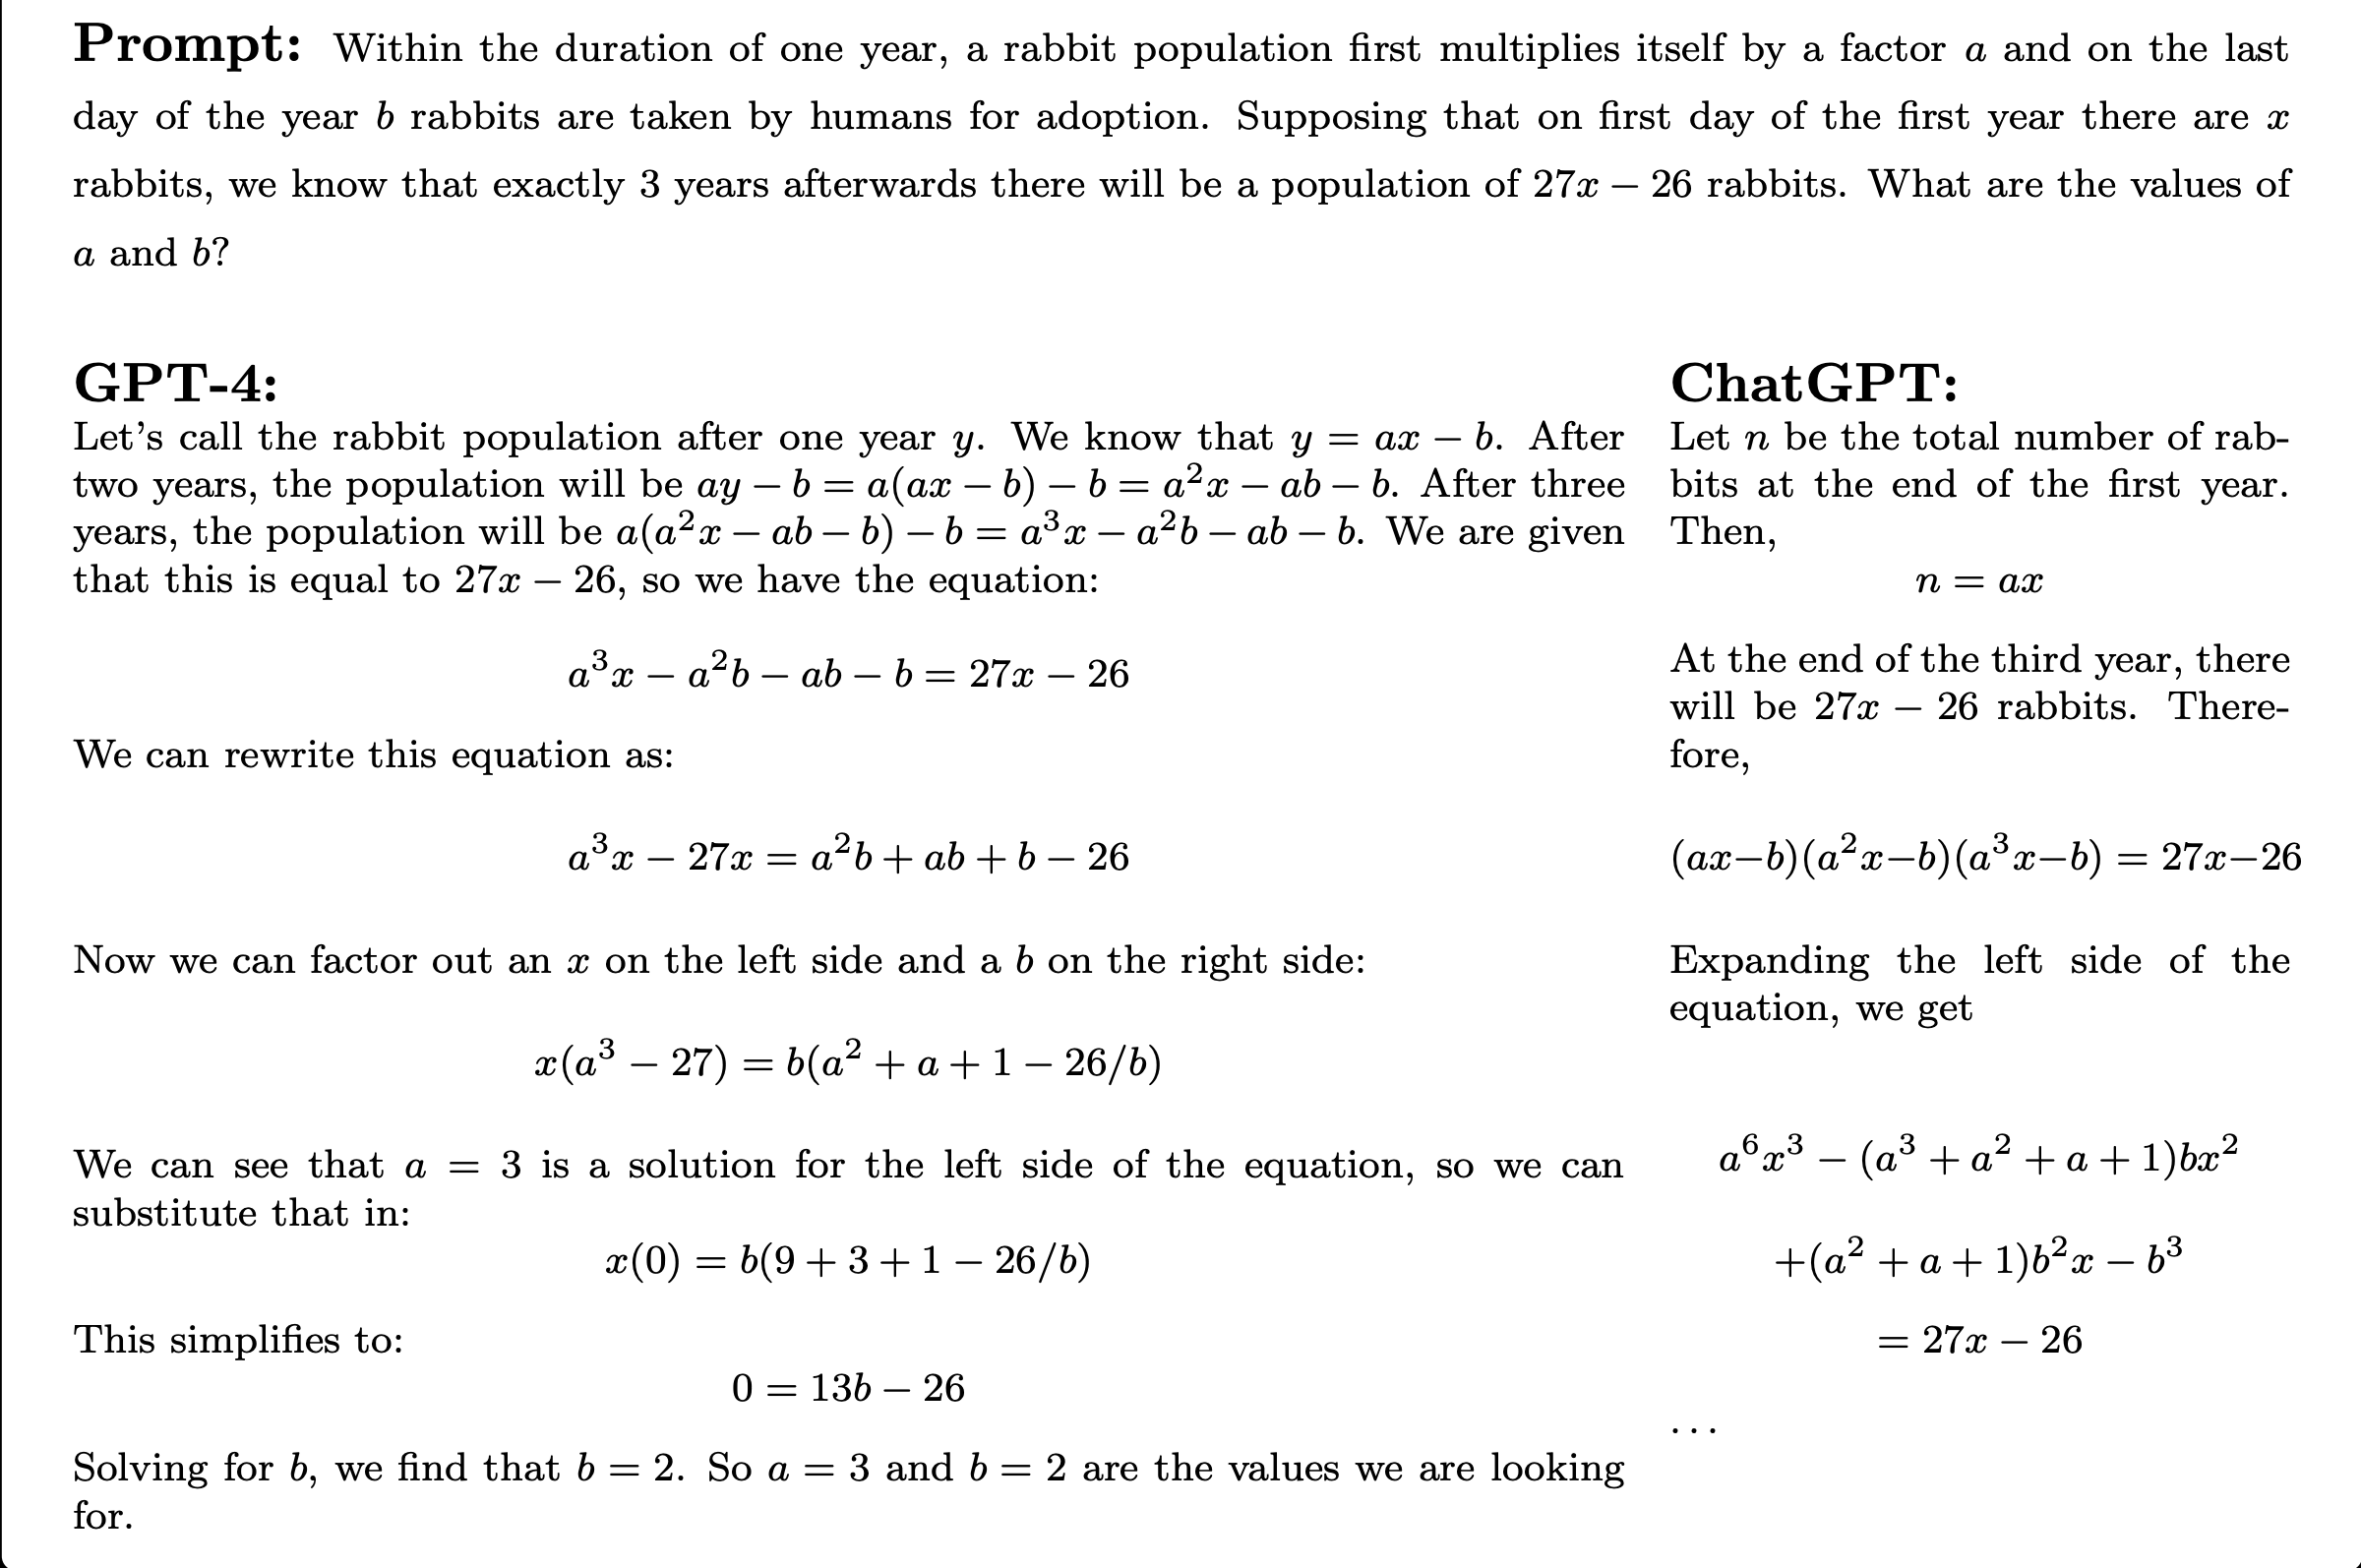
\includegraphics[width=0.50\textwidth]{images/math_explanation.png}
       \caption{\enquote{At one point, the model assumes that the two sides of the equation need to be zero, which relies on an implicit assumption
       that the equation must have a solution. This turns out to be correct, but the reasoning is inaccurate}\cite{bubeck2023sparks}.}       
       \label{fig:image1}
   \end{figure}
   
        Given ChatGPT's limitations in reasoning, it is better suited as a search-engine-like tool, akin to a teacher's assistant (TA). At Georgia Tech, one of the best TAs for a master's program was an AI based on IBM's Watson \cite{popenici2017}. OpenAI CEO Sam Altman recently stated, 
        \enquote{[…] we're at the end of the era where it's gonna be these giant models, and we'll make them better in other ways}\cite{miller2023}, implying that more specialized LLMs are preferable for specific tasks, enabling certain sectors to benefit more than from a general AI. Exploring ChatGPT's potential for research and planning can enhance efficiency and workflow in various projects. IBM's Watson, for instance, already assists large corporations and has proven more accurate at diagnosing medical conditions than human doctors \cite{popenici2017}. With the specialization of AI to better suit the needs of either corporations or students in a master's program, one can dream if these AI systems can be interlocked/combined to create a more self-sufficient AI. Something more akin to a general intelligent being.

   \subsection{A Quick Overview of AutoGPT}


    
    \bibliography{references.bib}
\end{document}